\chapter{La qualité de service}\label{ch:qos}

\section{Présentation}

Les besoins de chaque flux de données peuvent être caractérisés par quatre principaux paramètres : la fiabilité (reliability) , le temps d'acheminement (delay), la gigue (jitter), et la bande passante (bandwidth).\\
Fiabilité  : quel est le taux de perte des paquets dans le réseau ?\\
Temps d'acheminement : quel est le temps d'acheminement des paquets de la source à la destination ?\\
Gigue : avec quelle régularité les paquets arrivent-ils au destinataire ?\\
Bande passante : quelle quantité d'information peut être transmise en un temps donné (débit) ?\\
    
Les besoins pour chaque paramètre dépendent de l'application :
\begin{table}[!h]
  \centering
  \begin{tabular}{|l|l|l|l|l|} 
   \hline
    Application & Fiabilité & Temps d'acheminement & Gigue & Bande passante \\
    \hline
    Email & Important & Faible & Faible & Faible\\
    \hline
    Transfert de fichier & Important & Faible & Faible & Moyen\\
    \hline
    Navigation web & Important & Moyen & Faible & Moyen\\
    \hline
    Connexion distante & Important & Moyen & Moyen & Faible\\
    \hline
    Audio à la demande & Faible & Faible & Important & Moyen\\
    \hline
    Vidéo à la demande & Faible & Faible & Important & Important\\
    \hline
    Téléphonie & Faible & Important & Important & Faible\\
    \hline
    Vidéoconférence & Faible & Important & Important & Important\\
    \hline
  \end{tabular}
  \caption{Exemples des besoins de différentes applications. \cite{Tanenbaum2003}}
\end{table}

C'est pourquoi il est important de faire de la qualité de service en fonction du type d'application visée.\\

Il existe différentes techniques pour obtenir une bonne QoS :\\

\begin{itemize}
\item Surapprovisionnement (overprovisioning) :

Il s'agit de disposer de plus de ressources (espace de stockage, bande passante, débit...) que nécessaire, afin que tous les paquets puissent transiter sans la moindre attente. Cette solution est simple mais extrêmement coûteuse à mettre en place. D'autres solutions moins coûteuses permettent généralement d'atteindre les objectifs de Qualité de Service fixés. \\
\item La mise en mémoire tampon (buffering) :

Il s'agit de stocker les paquets d'un flux chez le destinataire avant de les délivrer. Cette solution permet de réduire la gigue (on peut contrôler la vitesse d'arrivée des paquets au destinataire) mais augmente le temps d'acheminement de la source à la destination.\\

\item La régulation de flux (traffic shaping) :

Il s'agit ici d'imposer à l'émetteur de transmettre ses paquets à une vitesse régulière (constante). Cela permet de diminuer la congestion dans le réseau (on empêche une machine d'envoyer une grande quantité de paquets en une seule fois).\\ Dans un protocole en mode connecté, l'émetteur et le récepteur peuvent aussi convenir des paramètres des flux de données à échanger lors de l'établissement de la connexion. Lorsque le destinataire reçoit un flux, et si le flux respecte la convention établie, le destinataire s'engage à transmettre les données dans les temps. Cette technique s'appelle la limitation du flux (traffic policing).\\

\item L'algorithme du seau percé (leaky bucket, Turner, 1986) :

Dans un seau percé rempli d'eau, peu importe la quantité d'eau dans le seau, le débit sortant ne varie pas; et lorsque le seau est plein, l'eau excédentaire est perdue. Dans cet algorithme, les paquets arrivants sont stockés dans une structure de file à taille fixée. A chaque tick d'horloge et si la file n'est pas vide, un paquet est défilé et envoyé. Lorsque la file est pleine, un paquet arrivant est jeté. Cet algorithme permet de fluidifier des échanges irréguliers ou limiter le débit dans un réseau.\\

\item L'algorithme du seau à jetons (token bucket) :

Cet algorithme est similaire à l'algorithme du seau percé mais plus flexible. Le seau percé contient un certain nombre de jetons. Un jeton est généré chaque intervalle de temps jusqu'à un certain seuil maximum du nombre de jetons total. Chaque paquet peut consommer un jeton pour être immédiatement transmis. Lorsqu'il n'y a plus de jetons disponibles, les paquets sont stockés comme dans l'algorithme du seau percé mais ne seront jamais jetés (a priori). Cet algorithme permet de mieux réguler le trafic lorsque de grande quantité de données arrivent à un routeur.\\

\item La réservation de ressource :

L'idée ici est de prévoir un chemin pour un certain flux de données (on créé une sorte de circuit virtuel), et de réserver toutes les ressources nécessaires sur cette route afin de garantir une bonne qualité de service pour ce flux passant par cette route. On pourra réserver de la bande passante, de l'espace de stockage ou encore de la capacité CPU dans les routeurs par exemple.\\

\item Le contrôle d'admission :

Lorsqu'un routeur reçoit un flux, il doit décider selon ses ressources disponibles immédiatement, de l'accepter ou de le rejeter. Cependant cette décision est compliquée car elle dépend de nombreux paramètres donnés (ou non) par l'émetteur. De plus, tous les routeurs sur le chemin de l'émetteur au destinataire peuvent avoir leurs propres contraintes.\\
Une solution est que l'émetteur transmette au destinataire les paramètres qu'il voudrait négocier (dont il aurait besoin) : nous les nommerons spécifications du flux. Tous les routeurs sur le chemin peuvent les examiner et les modifier si besoin mais seulement en réduisant le flux. Lorsque les spécifications ont été examinées par toutes les machines du chemin, elles sont adoptées : l'émetteur devra respecter ces spécifications lors de l'émission. Ainsi chaque routeur le long du chemin peut réserver les ressources nécessaires correspondantes.\\

\item Le routage proportionnel :

Au lieu de transmettre un flux arrivant, sur le meilleur chemin comme dans les algorithmes de routage classiques, il est possible de diviser ce flux et de le transmettre sur plusieurs chemins différents. Une méthode simple est de diviser le flux proportionnellement aux capacités des liens sortants.\\

\item L'ordonnancement de la transmission des paquets (packet scheduling) :

Un problème dans un routeur recevant plusieurs flux de données peut être qu'un flux utilise toutes les capacités du routeur et ainsi mette les autres flux dans une situation de famine. Il peut donc être intéressant d'implémenter des algorithmes d'ordonnancement des paquets arrivant dans un routeur.\\
L'algorithme du Fair queueing proposé par John Nagle en 1987 peut être une première solution : on associe une structure de file à chaque flux de données. Puis on défile et on transmet un paquet par file, file après file. Ainsi chaque flux est géré de manière équitable par le routeur.\\
Le problème de cet algorithme est qu'il est impossible de gérer des priorités différentes pour les flux. La solution est l'algorithme du Weighted fair queueing : une priorité (un poids) est affectée à chaque flux et on traite pour chaque file un nombre de paquets (ou un nombre d'octets) proportionnel à la priorité de la file.

\end{itemize}


    
\section{La qualité de service dans l'IPv6 \cite{Archier2012}}

Deux champs de l'en-tête IPv6 peuvent être utilisés pour la qualité de service : le champ Traffic Class (RFC 2474) et le champ Flow label, selon le type de système.
On peut distinguer deux types de système :
\begin{itemize}
\item Integrated Services : le but est de réserver les ressources de bout en bout d'une connexion
\item Differentiated Services (DiffServ) : la réservation de ressource se fait routeur par routeur, pas de réservation de ressources de bout ent bout
\end{itemize}

\subsection{Systèmes de type Integrated Services : le champ Flow Label}
Ici le but est de réserver les ressources de bout en bout, donc chaque routeur doit avoir des critères différents pour traiter chaque flux. Un routeur doit analyser chaque paquet pour savoir à quel flux il appartient. La même politique de QoS sera appliquée à tous les paquets d'un flux. L'entete IPv6 dispose pour cela du champ Flow Label.

    Le champ Flow label(codé sur 20 bits) et le champ Adresse Source identifient de manière unique un groupe de paquets (un flux). Ainsi, tous les paquets du même flux sont traités d'une manière identique par les routeurs, et donc plus rapidement.  
    
    Le Flow Label est assigné par le noeud source du flux. Il peut y avoir plusieurs flux entre deux noeuds en parallèle. Le Flow Label doit être choisi au hasard dans l'intervalle [00001;FFFFF].
    
    Lors d'une communication, dans un premier temps une phase de réservation de ressources est effectuée par le protocole RSVP (Ressource Reservation Protocol). Puis il y a transmission des paquets de données dans laquelle le Flow Label est utilisé pour classifier le paquet transmis.
    
    La transmission se déroule comme suit : 
    \begin{itemize}
    \item Connexion établie de A vers B
    \item B envoie une requête RSVP vers A : tous les routeurs sur le chemin réservent les ressources demandées si disponibles
    \item A renvoie un acquittement RSVP vers B
    \item A transmet ses paquets de données à B
    \end{itemize}

	L'intérêt d'utiliser le champ Flow Label comme marqueur de flux est que les routeurs n'ont plus à décoder la charge du paquet pour déterminer le flux auquel appartient le paquet. Le traitement et le routage des paquets est ainsi accéléré pour une QoS particulière.
    
\subsection{Systèmes de type DiffServ : le champ Traffic Class}
	\label{diffserv}
	Ici, le mécanisme est différent, le traitement se fait routeur par routeur (Per Hop Behavior : PHB). Ce type de système est plus simple à mettre en oeuvre et donc plus utilisé aujourd'hui.
    
    Le fonctionnement est le suivant : la source marque le paquet en positionnant certains bits du marqueur DSCP (Differentiated Service Code Point).
    Les routeurs recevant ce paquet le traite comme prioritaire sur ceux n'ayant aucun marquage ou des valeurs de DSCP inférieures.
    
    Le champ Traffic Class est aussi appelé DS field (Differentiated Service field): il remplace le champ Type of Service de l'IPv4. Il est codé sur 8 bits. Il permet de définir une classe ou une priorité au paquet pour un traitement spécifique.
    
    \begin{figure}[h]
    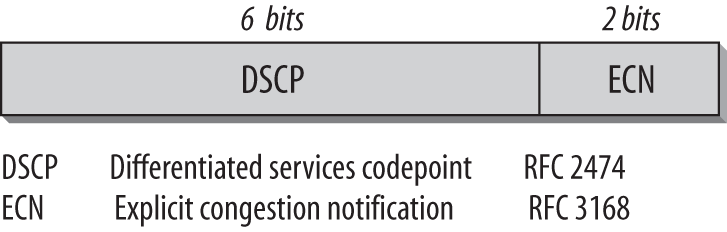
\includegraphics[width=250px]{figures/trafficclass.png}
    \centering
    \caption{Structure du champ Traffic Class. \cite{Hagen2014}}
    \label{paquet_traffic_class}
    \end{figure}
	
    
    Les 6 premiers bits définissent la valeur du DSCP  qui détermine la gestion des priorités du traffic ou per-hop behavior (PHB) de chaque routeur. 
    
    Le PHB détermine comment les paquets seront transmis par le routeur.
    Le PHB par défaut est codé par la suite : 000000. Il correspond au best-effort forwarding behavior c.a.d. que le réseau transmettra ces paquets sans aucune priorité et utilisera les ressources disponibles pour les transmettre.
    
    \begin{table}[!h]
  \centering
  \begin{tabular}{|l|l|l|} 
   \hline
    Groupe & Format du Codepoint & Politique d'affectation\\
    \hline
    1 & xxxxx0 & Usage standard \\
    \hline
    2 & xxxx11 & Usage expérimental ou local\\
    \hline
    3 & xxxx01 & Usage expérimental ou local; Ou en complément du groupe 1\\
    \hline
  \end{tabular}
  \caption{Groupes de Codepoints.}
\end{table}

    3 groupes de Code Points sont définis : xxxxx0 pour des PHB standardisés, xxxx11 pour un usage expérimental ou local et xxxx01 pour un usage expérimental ou local ou en supplément du groupe xxxxx0 si il est entièrement utilisé.
    
    Les 2 derniers bits du champ Traffic Class sont utilisés pour la notification explicite de congestion (ECN). Ces bits sont présents dans IPv4 et IPv6.

\subsection{Le champ HopByHop}
    Le champ HopByHop dans l'entete des options peut aussi être utilisé pour transporter un message d'alerte routeur (Multicast Listener Discovery message, RSVP message....). De cette manière, le paquet peut être traité plus rapidement car il est inutile d'analyser des entetes d'autres protocoles de plus haut niveau par les routeurs intermédiaires pour détecter que c'est un paquet message.
    
\subsection{Absence de NAT}
	La Network Address Translation (NAT) n'existe plus en IPv6 car suffisament d'adresses IP sont disponibles et donc la NAT n'est plus nécessaire. De cette manière, la QoS n'est plus arrêtée par la NAT et peut s'étendre sur des réseaux plus importants.